\documentclass[a4paper,12pt,french]{article}

\usepackage{../../Style}

\renewcommand\tabularxcolumn[1]{m{#1}}

\setcounter{section}{1}

\pagestyle{empty}

\begin{document}

\section{Modes de générations de suites}

Une suite peut être générée de trois manières différentes:

\subsection{Par une expression explicite}

Il s'agit d'une suite vérifiant $u_n=f(n)$ avec $f$ une fonction.

\begin{ex}
On se donne la suite $(u_n)$ définie pour tout entier naturel $n$ par $u_n=n^2-3n$.

\begin{center}
\begin{tabularx}{0.7\linewidth}{ 
  | >{\centering\arraybackslash}c 
  | >{\centering\arraybackslash}X
  | >{\centering\arraybackslash}X
  | >{\centering\arraybackslash}X
  | >{\centering\arraybackslash}X
  | >{\centering\arraybackslash}X
  | >{\centering\arraybackslash}X
  | >{\centering\arraybackslash}X| } \hline
$n$ & 0 & 1 & 2 & 3 & 4 & 5 & 6\\ \hline
$u_n$ &  & & & & & &\rule[-7pt]{0pt}{30pt} \\ \hline
\end{tabularx}
\end{center}

\end{ex}

\subsection{Par une relation de récurrence}

On donne le premier terme $u_0$ de la suite puis une relation permettant de calculer le terme suivant à partir du précédent.

\begin{exs} \
\begin{itemize}
\item On se donne la suite $(v_n)$ dont le premier terme est $1$ et dont le terme suivant est obtenu en doublant le terme précédent. On a alors $v_0= 1$, $v_1$ est le double de $v_0$ donc $v_1=2 \times v_0=2$, puis de même $v_3=4,\ v_4=8,\ v_5=16 \ldots$ Pour résumer cette relation, on note $u_{n+1} = 2 \times u_n$.
\end{itemize}

\begin{center}
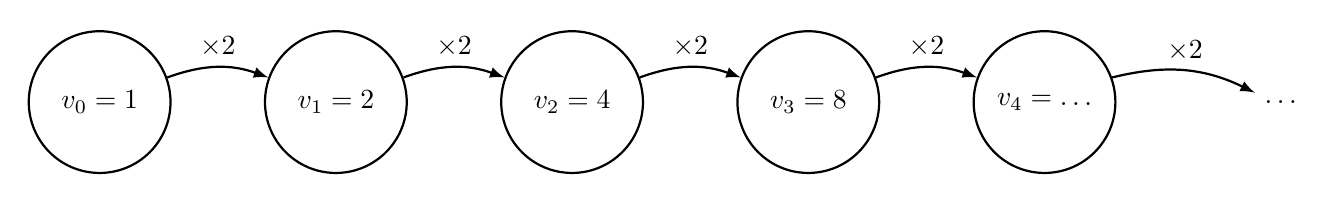
\begin{tikzpicture}[scale=1]
\node[draw,circle,thick, minimum size=18mm] (W0) at (-3,0) {$v_0=1$};
\node[draw,circle,thick, minimum size=18mm] (W1) at (0,0) {$v_1=2$};
\node[draw,circle,thick, minimum size=18mm] (W2) at (3,0) {$v_2=4$};
\node[draw,circle,thick, minimum size=18mm] (W3) at (6,0) {$v_3=8$};
\node[draw,circle,thick, minimum size=18mm] (W4) at (9,0) {$v_4=\ldots$};
\node (W5) at (12,0) {$\ldots$};
\draw[->,>=latex,thick] (W0) to[bend left=20] node[midway,above]{$\times 2$} (W1);
\draw[->,>=latex,thick] (W1) to[bend left=20] node[midway,above]{$\times 2$} (W2);
\draw[->,>=latex,thick] (W2) to[bend left=20] node[midway,above]{$\times 2$} (W3);
\draw[->,>=latex,thick] (W3) to[bend left=20] node[midway,above]{$\times 2$} (W4);
\draw[->,>=latex,thick] (W4) to[bend left=20] node[midway,above]{$\times 2$} (W5);
\end{tikzpicture}
\end{center}

\begin{itemize}
\item Soit $(w_n)$ la suite définie par $w_0=0$ et pour tout entier naturel $n$, $w_{n+1}=2w_n+1$. Alors $w_1=2w_0+1=2 \times 0 + 1=1 \ , \ w_2=2w_1+1=3 \ , \ w_3=7 \ldots$
\end{itemize}

\begin{center}
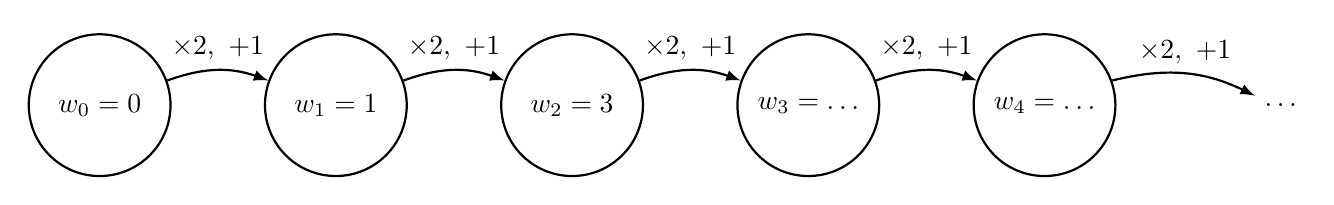
\begin{tikzpicture}[scale=1]
\node[draw,circle,thick, minimum size=18mm] (W0) at (-3,0) {$w_0=0$};
\node[draw,circle,thick, minimum size=18mm] (W1) at (0,0) {$w_1=1$};
\node[draw,circle,thick, minimum size=18mm] (W2) at (3,0) {$w_2=3$};
\node[draw,circle,thick, minimum size=18mm] (W3) at (6,0) {$w_3=\ldots$};
\node[draw,circle,thick, minimum size=18mm] (W4) at (9,0) {$w_4=\ldots$};
\node (W5) at (12,0) {$\ldots$};\draw[->,>=latex,thick] (W0) to[bend left=20] node[midway,above]{$\times 2,\ + 1$} (W1);
\draw[->,>=latex,thick] (W1) to[bend left=20] node[midway,above]{$\times 2,\ + 1$} (W2);
\draw[->,>=latex,thick] (W2) to[bend left=20] node[midway,above]{$\times 2,\ + 1$} (W3);
\draw[->,>=latex,thick] (W3) to[bend left=20] node[midway,above]{$\times 2,\ + 1$} (W4);
\draw[->,>=latex,thick] (W4) to[bend left=20] node[midway,above]{$\times 2,\ + 1$} (W5);
\end{tikzpicture}
\end{center}

\end{exs}

\subsection{Par une définition plus abstraite}

\begin{ex}
Soit $(w_n)$ la suite des chiffres de l'écriture décimale de $\sqrt 2 = 1.414213\ldots$. Alors $w_0=1 \ , \ w_1=4 \ , \ w_2=\ldots \ , \ w_3=\ldots \ , \ w_4=\ldots \ , \ \ldots$
\end{ex}

\subsection{Un exemple pour résumer}

On se donne les trois suites suivantes:
\begin{itemize}
\item La suite $u$ des nombres pairs.
\item La suite $v$, qui vérifie pour tout $n \in \N, u_n=2n$.
\item La suite $w$ telle que $w_0=0$, et pour tout $n \in \N, w_{n+1}=2 \times w_n$.
\end{itemize}

\begin{center}
\begin{tabularx}{0.7\linewidth}{ 
  | >{\centering\arraybackslash}c 
  | >{\centering\arraybackslash}X
  | >{\centering\arraybackslash}X
  | >{\centering\arraybackslash}X
  | >{\centering\arraybackslash}X
  | >{\centering\arraybackslash}X
  | >{\centering\arraybackslash}X
  | >{\centering\arraybackslash}X| } \hline
$n$ & 0 & 1 & 2 & 3 & 4 & 5 & 6\\ \hline
$u_n$ & & & & & & & \rule[-7pt]{0pt}{30pt} \\ \hline
$v_n$ & & & & & & & \rule[-7pt]{0pt}{30pt} \\ \hline
$w_n$ & & & & & & & \rule[-7pt]{0pt}{30pt} \\
\hline
\end{tabularx}
\end{center}

En fait, on peut montrer que ces trois suites sont \makebox[3cm]{\dotfill}

\begin{comment}
On se donne la suite $u$ des nombres pairs. Cette définition est abstraite. On pourra vérifier que les définitions suivantes génèrent la même suite:
\begin{itemize}
\item Pour tout $n \in \N, u_n=2n$
\item $u_0=0$ et pour tout $n \in \N, u_{n+1}=u_n+2$.
\end{itemize}

\begin{center}
\begin{tabularx}{\linewidth}{ 
  | >{\centering\arraybackslash}c 
  | >{\centering\arraybackslash}X
  | >{\centering\arraybackslash}X
  | >{\centering\arraybackslash}X
  | >{\centering\arraybackslash}X
  | >{\centering\arraybackslash}X
  | >{\centering\arraybackslash}X
  | >{\centering\arraybackslash}X| } \hline
$n$ & 0 & 1 & 2 & 3 & 4 & 5 & 6\\ \hline
Définition abstraite de $u_n$ & & & & & & & \rule[-7pt]{0pt}{30pt} \\ \hline
Définition explicite de $u_n$ & & & & & & & \rule[-7pt]{0pt}{30pt} \\ \hline
Définition par récurrence de $u_n$ & & & & & & & \rule[-7pt]{0pt}{30pt} \\
\hline
\end{tabularx}
\end{center}
\end{comment}

\end{document}